\section{The System}
\label{sec:system}

\begin{figure}[t]
\centering
% Figure 1: one task, from the request to the answer, as a sequence of
% messages between the child's card, the chat's model, the service and the
% parent's Google Drive, on the path where the task is accepted. The paper's
% preamble defines \System and loads TikZ; arrows use only the tips TikZ has
% without a library. Each party's column is set once, below, and every arrow
% stands on those columns.
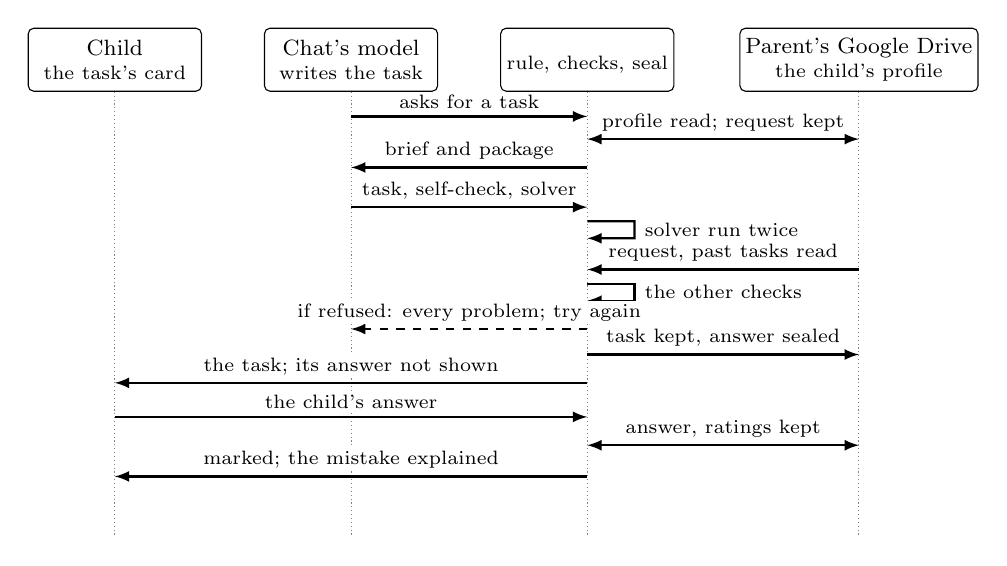
\begin{tikzpicture}[
  y=0.72cm,
  font=\footnotesize,
  >=latex,
  party/.style={draw, rounded corners=2pt, align=center, minimum width=22mm, minimum height=8mm, inner sep=2pt},
  life/.style={densely dotted, gray},
  msg/.style={->, thick},
  back/.style={->, thick, dashed},
  trip/.style={<->, thick},
  note/.style={font=\scriptsize, align=center, fill=white, inner sep=1pt, above=1.5pt},
  aside/.style={font=\scriptsize, align=left, right},
]
  \def\xCard{0}\def\xModel{3.0}\def\xService{6.0}\def\xDrive{9.45}

  % The four parties, left to right, and their lifelines.
  \node[party] (card)    at (\xCard,0)    {Child\\[-1pt]{\scriptsize the task's card}};
  \node[party] (model)   at (\xModel,0)   {Chat's model\\[-1pt]{\scriptsize writes the task}};
  \node[party] (service) at (\xService,0) {\System\\[-1pt]{\scriptsize rule, checks, seal}};
  \node[party] (drive)   at (\xDrive,0)   {Parent's Google Drive\\[-1pt]{\scriptsize the child's profile}};
  \foreach \p in {card, model, service, drive}
    \draw[life] (\p.south) -- ++(0,-7.85);

  % The request: the rule reads the profile, keeps the request in it and
  % writes the brief.
  \draw[msg]  (\xModel,-1.0)    -- node[note] {asks for a task} (\xService,-1.0);
  \draw[trip] (\xService,-1.4)  -- node[note] {profile read; request kept} (\xDrive,-1.4);
  \draw[msg]  (\xService,-1.9)  -- node[note] {brief and package} (\xModel,-1.9);

  % The task: its solver runs before the profile is read; the other checks
  % need the request and the child's past tasks; a refused task goes back.
  \draw[msg]  (\xModel,-2.6)    -- node[note] {task, self-check, solver} (\xService,-2.6);
  \draw[msg]  (\xService,-2.85) -- ++(0.6,0) -- node[aside] {solver run twice} ++(0,-0.3) -- (\xService,-3.15);
  \draw[msg]  (\xDrive,-3.7)    -- node[note] {request, past tasks read} (\xService,-3.7);
  \draw[msg]  (\xService,-3.95) -- ++(0.6,0) -- node[aside] {the other checks} ++(0,-0.3) -- (\xService,-4.25);
  \draw[back] (\xService,-4.75) -- node[note] {if refused: every problem; try again} (\xModel,-4.75);
  \draw[msg]  (\xService,-5.2)  -- node[note] {task kept, answer sealed} (\xDrive,-5.2);
  \draw[msg]  (\xService,-5.7)  -- node[note] {the task; its answer not shown} (\xCard,-5.7);

  % The answer: unsealed, marked and explained; the ratings move.
  \draw[msg]  (\xCard,-6.3)     -- node[note] {the child's answer} (\xService,-6.3);
  \draw[trip] (\xService,-6.8)  -- node[note] {answer, ratings kept} (\xDrive,-6.8);
  \draw[msg]  (\xService,-7.35) -- node[note] {marked; the mistake explained} (\xCard,-7.35);
\end{tikzpicture}

\caption{One accepted task, from request to answer: the model writes it and the service checks it; a refused task goes back with every problem found (dashed). The profile, with the sealed answer, lives in the parent's Google Drive.}
\label{fig:flow}
\end{figure}

Each mechanism of the service serves a learning goal, and at the pinned commit all of them are built: every problem new, by a near-duplicate check against reference tasks and the child's past ones; ``slightly harder'', by a corridor of predicted success of \statr{product}{corridor_low}{2}--\stat{product}{corridor_high}; diagnosable mistakes, by a trap of a closed catalog behind each wrong option, explained; the answer not given away, by a seal until the child answers; and a checked key, by the model's own solver run twice.

\paragraph{Who does what.} Figure~\ref{fig:flow} follows one task. A deterministic rule reads the child's profile and builds a brief: the goal, the topic, a grade level and difficulty on one ladder, a setting and the child's \statword{product}{brief_traps} most frequent traps in the topic; the model may ask for something else, but must say why. With the brief comes a package --- the corridor, the trap catalog, the skills the task may not use, the child's grade, interests and the parent's notes, \statword{product}{package_examples} reference tasks, solver templates and a guide --- which carries no pseudonym and fits \stat{product}{package_budget_kib}\,KiB. The model hands in the question, \statword{product}{options} options, the key, a hint, a solution, each wrong option's trap and explanation, a self-check and a solver; a refused task goes back with every problem found, \statword{product}{max_attempts} attempts a request. The card shows the question, the drawing, the options and the hint; once the child answers, the service unseals the task, marks it, explains a wrong option's mistake and updates the ratings.

\paragraph{Architecture and content.} The service is a single Go binary with no database, on Google Cloud Run, that keeps nothing of a child between requests. The profile is a JSON file in the parent's own Google Drive, reached with the parent's token through the service's own OAuth server. It speaks the Model Context Protocol, revision \stat{product}{mcp_revision}, without sessions, through \statword{product}{mcp_tools} tools, calls no language model and depends on no model provider's SDK; each card is an MCP Apps page~\cite{mcpapps2026} that names no outside domain. The catalogs hold \stat{product}{topics} topics, \stat{product}{traps} traps --- typical mistakes, such as answering a different question --- and \stat{product}{skills} skills. The \stat{product}{reference_tasks} reference tasks, \stat{product}{reference_tasks_1_2}, \stat{product}{reference_tasks_3_4} and \stat{product}{reference_tasks_5_6} for grades \stat{product}{grade_level_1}, \stat{product}{grade_level_2} and \stat{product}{grade_level_3}, each have a solver and a trap behind each wrong option. An earlier study of sources chose problem books in the public domain, whose copyright has expired; Claude wrote the tasks from their ideas at our request, in wording of its own, and we checked them. In first runs with a real model, Claude Sonnet 5 wrote \stat{ledger}{live_tasks} tasks over \stat{ledger}{live_handins} hand-ins, \stat{ledger}{live_first_attempt} accepted at the first attempt, and a trial series of \statword{product}{trial_answers} tasks went through in Claude's web client. Such runs are too few to measure anything, so our evaluation runs offline.
